\documentclass{article}
\usepackage{amssymb}
\usepackage{wasysym}
\usepackage{graphics}
\usepackage{bm}
\usepackage{psfig}
\newcommand{\bc}{\begin{center}}
\newcommand{\ec}{\end{center}}
\newcommand{\be}{\begin{equation}}
\newcommand{\ee}{\end{equation}}
\newcommand{\bea}[1]{\begin{eqnarray}\label{#1}}
\newcommand{\eea}{\end{eqnarray}}
\newcommand{\bua}{\begin{eqnarray*}}
\newcommand{\eua}{\end{eqnarray*}}
\newcommand{\infint}{\int_{-\infty}^{\infty}}
\newcommand{\dd}[2]{{{d#1}\over{d#2}}}
\newcommand{\ddt}[1]{\dd{#1}{t}}
\newcommand{\dddt}[1]{\dd{^2#1}{t^2}}
\newcommand{\aver}[1]{\langle{#1}\rangle}
\def\cl#1{{\cal #1}}               % for caligrafic letters
\def\labs{\mid\!}
\def\rabs{\!\mid}
\begin{document}
\setcounter{section}{9}
\newcounter{count}
\setcounter{count}{\value{enumi}}
\section{Spectroscopy}

Practical telescopes are usually based upon one or other of two quite separate optical
principles --- interference and differential refraction. In reality, the author has never
seen a prism based spectrograph professionally used $\ldots$ There are also some 
hybrid designs according to Kitchin's {\it Astrophysical Techniques}. 

\subsection{Diffraction Gratings}

The operating principle of diffraction gratings relies on the effects of diffraction 
and interference of light waves. 

A diffraction grating can be modeled as a finite series of alternating transparent 
and opaque, long, parallel stripes. Let there be $N$ transparent and opaque stripes 
each of width $a\gg\lambda$. We can idealize them as infinitely long so their diffraction
pattern is one-dimensional.

The idealized $N$-slit grating can be considered as an infinite series of $\delta$-functions with separation $2a$ convolved with the transmission function
for a single slit,
\[
\int_{-\infty}^{\infty}\left[\sum_{n=-\infty}^{\infty}\delta(y-2an)\right] t_1(x-y)dy,
\]
that is multiplied by the global aperture function of the size of the grating
\bua
H(x)&=&1 \qquad \labs x\rabs<Na \\
      &=&0 \qquad \labs x\rabs>Na.
\eua
In total this gives an aperture function for the entire grating 
\[
t(x)=\left(\int_{-\infty}^{\infty}\left[\sum_{n=-\infty}^{\infty}\delta(y-2an)\right]t_1(x-y)dy\right)H(x)
\]
The final pattern is then given by remembering that $\psi_{\cl{P}}$ is given by the 
Fourier transform of $t(x)$
\[
\psi_\cl{P}({\theta)\propto\int e^{-ikx\theta}}t({x})dx.
\]
The convolution theorem says that the Fourier transform of two functions is the product
of the functions' Fourier transforms, and conversely. The diffraction pattern of of the infinite series of $\delta$-functions with spacing $2a$ is itself an infinite series of $\delta$-functions, but with the reciprocal spacing ${2\pi/(2ka)}={\lambda/2a}$. This
is multiplied by the Fourier transform of the single slit, and then convolved with the
Fourier transform of $H(x)$, $\bar{H}(\theta)\propto{\rm sinc}(Nka\theta)$. The 
diffracted energy flux is $\labs\psi_{\cl{P}}\rabs^2$: what the grating does is channel the
incident radiation into a few equally spaced beams with directions $\theta={\pi m/ka}$,
where $m$ is is an integer known as the {\it order} of the beam. Each of these beams 
has the shape given by $\labs\bar{H}(\theta)\rabs^2$: a sharp centered peak with a
half width (distance from the center of the peak to the first null of the intensity)
${\lambda/2Na}$, followed by a set of {\it side lobes} whose intensities are $\propto N^{-1}$. 

A spectrograph can therefore be built based on the fact that the deviation angle $\theta={\pi m/ka}$ of these beams are proportional to $k^{-1}={\lambda/2\pi}$.
We can find the wavelength resolution of of this (idealized) grating by focusing attention
the $m$'th order beams at two wavelengths $\lambda$ and $\delta\lambda$ located
at $\theta={m\lambda/2a}$ and $m(\lambda+\delta\lambda)/2a$. We can distinguish
the beams from each other when their separation $\delta\theta={m\delta\lambda/2a}$
is at least as large as the angular distance ${\lambda/2Na}$ between the maximum
of each beam's diffraction pattern and its first minimum:
\[ 
{\lambda\over\delta\lambda}\lesssim\cl{R}\equiv Nm
\]
$\cl{R}$ is called the gratings {\it chromatic resolving power}.

In Kitchin's {\it Astrophysical Techniques} the small angle approximation 
($\theta\approx\sin\theta$) is not used, and therefore a slightly different expression for the fringe pattern arises
\[
I(\theta)\propto\left[{\sin^2\left({\pi D\sin\theta/\lambda}\right) 
               \over\left({\pi D\sin\theta/\lambda}\right)^2}\right]
                 \left[{\sin^2\left({N\pi d\sin\theta/\lambda}\right) 
               \over\sin^2\left({\pi d\sin\theta/\lambda}\right)}\right]
\]
where now $D$ is the size of an aperture and $d$ is the distance between the apertures.
The angular positions of the principal maxima are given by
\[
\sin\theta=({m\lambda/d})
\]
and the zero intensities are found at 
\[
\sin\theta=({m'\lambda/Nd})
\]
excluding those positions $m'=mN$ that are the positions of the principle maxima.
The angular width of a principal maximum is therefore (since 
\[ {d\theta\over dm'}={\lambda\over Nd\cos\theta}\]
and the change in $m'$ is 2) given by
\[ W={2\lambda\over Nd\cos\theta}. \]
Thus, the width of a fringe is proportional to $N^{-1}$, while its peak intensity is proportional to $N^2$. The distance from the peak to the first zero $W'$ is half of 
this and the spectral resolution is then
\bua
W_\lambda&=&W'{d\lambda\over d\theta}
 ={\lambda\over Nd\cos\theta}{d\cos\theta\over m} \\
&=&{\lambda\over Nm}
\eua
The spectral resolution improves with the order. The chromatic resolving power is again
\[\cl{R}={\lambda\over W_\lambda}=Nm.\]
Note that it is independent of the width and the spacing of the apertures. Note that at high order the spectra are overlapping. The difference in wavelength between two superimposed wavelengths from adjacent spectral orders is called the free spectral 
range, $\Sigma$. If $\lambda_1$ and $\lambda_2$ are two such superimposed 
wavelengths then
\[ \sin^{-1}\left[{m\lambda_1\over d}\right]=\sin^{-1}\left[{(m+1)\lambda_2\over d}\right],\]
or for small angles
\[ \Sigma=\lambda_1-\lambda_2\approx{\lambda_2\over m}. \]
For small $m$, $\sigma$ is large. 

\begin{enumerate}
\item The overlapping of multiple orders means that some method --- a
  blocking filter or a detector of limited spectral sensitivity ---
  must be used to eliminate unwanted orders. Suppose we limit
  the response of a detector to wavelenghts shorter than some
  $\lambda_{\rm max}$. If we attempt to observe the spectrum in order
  $m$ with this detector, the spectrum from order $m+1$ overlaps
  $\lambda_{\rm max}$ so that photons of wavelength 
\[
\lambda_{m+1}=\frac{m}{(m+1)}\lambda_{\rm max}
\]
are deposited at the same $\theta$ location. We therefore would insert
a filter to block all light with wavelengths shorter than
$\lambda_{\rm max}$ to eliminate the overlap. What is the free spectral range at
  $\lambda_{\rm max}$? Explain why the free spectral for a particular
  order, $m$, and maximum wavelength $\lambda_{\rm max}$ is not
  restricted by overlapping light from order $m-1$.
\item Compute the free spectral range of grating orders 50, 100, and
  101 if $\lambda_{\rm max}=600$~nm in each case.
\setcounter{count}{\value{enumi}} 
\end{enumerate}

Some spectroscopes, such as those based on Fabry-Perot etalons and echelle gratings, 
operate at very high spectral order and both of the overlapping wavelengths may be
desired. Then it is necessary to use a cross disperser so that the final spectrum 
consists of a two-dimensional array of short sections of the spectrum.

Typical gratings for astronomical use have between 1000 and $50\,000$ grooves in total.
They are used at order ranging from one up to two hundred or so. Thus the spectral 
resolutions range from $10^3$ to $10^5$. Diffraction gratings can be used in either 
reflection or transmission modes, most astronomical spectroscopes are based on reflection gratings. Often, the grating is inclined to the incoming beam of light, in which
case a constant term, $d\sin i$, is added to the path differences, where $i$ is the angle
made by the incoming beam to the normal of the grating. Thus we find
\[
\theta=\sin^{-1}\left[\left({m\lambda\over d}\right)-\sin i\right]
\]
often called the grating equation.

The basic setup of a spectroscope is that the grating is illuminated by parallel light
that is usually obtained by placing a slit at the focus of a collimating lens (but sometimes by allowing light from a very distant object to fall directly on the grating).
After reflection from the grating, the light is focused by the imaging lens (camera lens)
to form the required spectrum. The collimator and imaging lens may be simple lenses or they may be achromats or mirrors.

\begin{enumerate}
\setcounter{enumi}{\value{count}}
\item Make a sketch of such a spectroscope, indicating the focal lengths
of the collimator, $f_1$, and imaging (camera) lens, $f_2$, the position of
the entrance slit, the grating and the detector. Also make a sketch
of the expected input and output images of the spectrograph, both
parallell and perpendicular to the plane of the sketch.
\item Show, or explain, why the width of a monchromatic image of the
  entrance slit is given by $S={sf_2/f_1}$ where $s$ is the width of
  the entrance slit.
\setcounter{count}{\value{enumi}} 
\end{enumerate}

If $x$ is the linear distance along the spectrum from some reference point, then we have
for an achromatic imaging element of focal length $f_2$
\[
{dx\over d\lambda}=f_2{d\theta\over d\lambda}
\]
where $\theta$ is small. Thus, the linear dispersion within each spectrum is given by
\[
{dx\over d\lambda}=\pm{mf_2\over d\cos\theta},
\]
or, since $\theta$ varies little over an individual spectrum
\[
{dx\over d\lambda}\approx {\rm constant}.
\]
More commonly, the reciprocal linear dispersion, ${d\lambda/dx}$, is used. It usually 
has values in the range $10^{-7}$ to $10^{-5}$.

The resolving power of a spectroscope is limited by the spectral resolution of the grating,
the resolving power of the optics, and by the projected slit width. The spectrum is formed
from an infinite number of monochromatic images of the entrance slit. The width of 
these images, $S$, is given by
\[
S=s{f_2\over f_1}
\]
where $s$ is the slit width, $f_1$ is the collimator's focal length and $f_2$ is the imaging element's focal length. The entrance slit must have a physical width of
$s_{\rm max}$ or less, if it is not to degrade the spectral resolution, where
\[
s_{\rm max}={\lambda f_1\over N d\cos\theta}.
\]

When the grating is fully illuminated, the imaging element will intercept a rectangular 
beam of light. The width of the beam, $D$, is given by $D=L\cos\theta$ where $L$ is 
the length of the grating and $\theta$ is the angle of the exit beam to the normal of the
plane of the grating. The diffraction limit is just that of a rectangular slit of width $D$:
the Rayleigh limit $W''$ is then given by 
\[
W''={f_2\lambda\over D}={f_2\lambda\over L\cos\theta}.
\]
Optimum resolution occurs when $S=W''$, {\it i.e.} when
\[ 
s={f_1\lambda\over D}={f_1\lambda\over L\cos\theta}.
\]

\noindent
{\it Blazing.} It is common to design a grating so that light is concentrated into a smaller
number of orders. In this technique, called blazing, the individual mirrors that comprise
the grating are angled so that they concentrate into a narrow sold angle. For instruments
based on on gratings at low orders, the angle of the mirrors is arranged so that the light
is concentrated into the spectrum to be used, and by this means 90\% efficiency can be
achieved. 

\noindent
{\it Shadowing.} If the incident and/or reflected light makes a large angle to the normal of
the grating, then the step-like nature of the surface will cause a significant fraction 
of the light to be intercepted by the vertical portions of the grooves, and so lost to the final spectrum. 

\noindent
{\it Rowland circle.} Curved reflection gratings are often used. By making the curve that of
an optical surface, the grating itself can be made to fulfill the function of the collimator
and/or the imaging element of the spectroscope, thus reducing light losses. The simplest optical principle employing a curved is due to Rowland. The slit, grating and 
spectrum all lie on a single circle called the Rowland circle. This has a diameter equal
to the radius of the curvature of the grating. 

\noindent
{\it Echelle gratings} By increasing the angle of a blazed grating, we obtain an echelle 
grating. This is illuminated more or less normally to the groove surfaces and therefore at
a very large angle to the normal to the grating. It is usually a very coarse grating ---
ten lines per millimeter or so --- so that the separation of the apertures $d$ is very large. The reciprocal linear dispersion
\[
{d\lambda\over dx}=\pm{d\cos\theta\over mf_2}
\]
is therefore also very large. Such gratings concentrate the light into many overlapping high-order spectra, and the resolution is very high. An echelle grating requires second
low dispersion grating or prism whose dispersion is perpendicular to that of the echelle
and is called a cross disperser in order to separate the orders. Alternately, one can use filters to remove unwanted orders.

\noindent
{\it Littrow spectroscopes} A type of arrangement often used for long focus spectroscopes in laboratory and solar work, is called the Littrow or auto-collimating spectroscope. A single lens, or occasionally a mirror, acts as both the collimator and imaging element.

\subsubsection{Ghosts and other anamolies}

A grating spectrum generally suffers from unwanted additional features superimposed upon the desired spectrum. Such features are usually much fainter than the main spectrum and are called ghosts. They arise from a variety of causes. They may be due
to overlapping spectra from higher or lower orders, or to the secondary maxima associated with each principal maximum. The first of these can be eliminated by the use
of filters since the overlapping ghosts are of different wavelengths. The second source
is usually unimportant since the secondary maxima are very weak when more that a few
tens of apertures are used, though they will contribute to the wings of the PSF. 
Of more general importance are the ghosts that arise through errors in the grating. 
Such errors most commonly take the form of periodic variations in the groove spacing.
A variation with a single period gives rise to {\it Rowland ghosts} that appear as faint
lines close to and on either side strong spectral lines. Their intensity is proportional to the square of the order of the spectrum. If the error is multi-periodic, then {\it Lyman ghosts} of strong lines may appear. These are similar to Rowland ghosts, except that they can be formed at large distances from the line that is producing them. 

Woods anamolies also sometimes occur, these are due to light that should go into spectral orders behind the grating reappearing with lower order spectra. They are rarely 
important in efficiently blazed gratings.

\subsection{Prisms}

Pure prism-based spectroscopes are rarely encountered today. However, they are used in 
conjunction with gratings in some modern instruments. Prisms are often used as cross-dispersers for high spectral order telescopes based upon echelle gratings or etalons, and may also be used non-spectroscopically for folding light beams.

When monochromatic light passes through an interface between two transparent isotropic
media at a fixed temperature, then we can apply Snell's law relating the angle of incidence, $i$, to the angle of refraction $r$ at that interface
\[ 
\mu_1\sin i=\mu_2\sin r
\]
where $\mu_1$ and $\mu_2$ are constants that are characteristic of the tow media. 
When $\mu_1=1$, {\i.e.} in a vacuum (but close enough in most gases including air), 
we have
\[
{\sin i\over\sin r}=\mu_2
\]
and $\mu_2$ is known as the refracting index of the second medium. Thus with a proper
second medium formed as a prism we can separate light into a spectrum. This is explained in great detail in Kitchin's {\it Astrophysical Techniques}.

\subsection{Interferometers}

\subsubsection{Michelson interferometer}

\begin{figure}[h]
  \centering  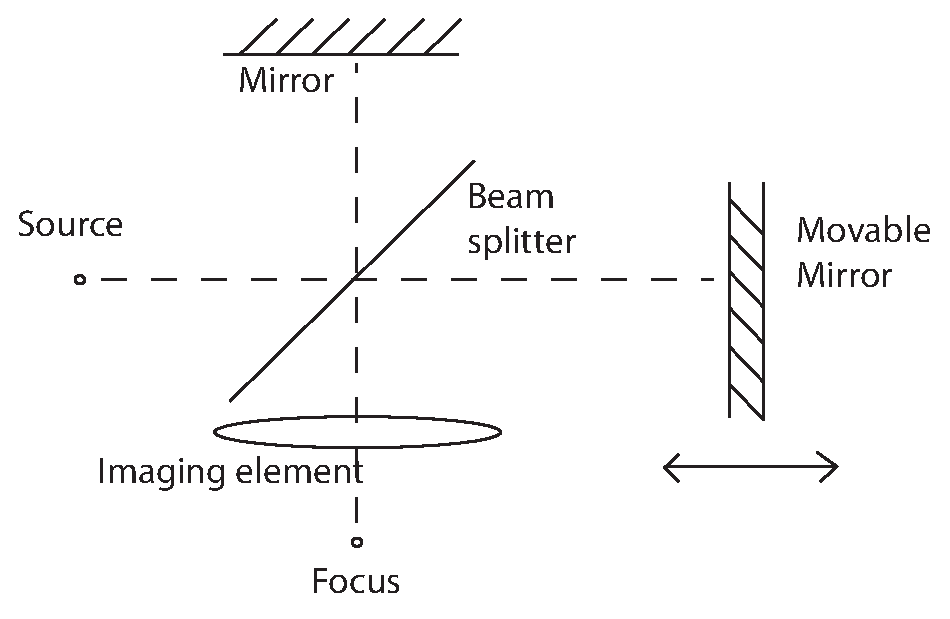
\psfig{file=michelson-interferometer.eps,width=0.95\textwidth}
  \caption{Optical pathway of a Michelson interferometer}
  \label{fig:michelson-interferometer}
\end{figure}

The Michelson interferometer is similar to the device used by Michelson and Morley to
try to detect the Earth's motion through the aether. The light from a source is split
into two beams by the beam splitter, and then recombined as shown in figure~\ref{fig:michelson-interferometer}. For a particular position of the movable mirror
and with a monochromatic source , there will be a path difference $\Delta P$ between the
two beams at focus. The flux at focus is then
\[
F_{\Delta P}=F_{\rm m}\left[1+\cos(k\Delta P)\right]
\]
where $F_{\rm m}$ is the maximum flux. When the mirror is moved the path difference will change and the final flux will pass through a series of maxima and minima. The change of the interference of the beam with itself is giving information on the wavelength of the beam $\lambda={2\pi/k}$. This will also be true for chromatic sources.

Consider a Michelson interferometer in which the path difference is $\Delta P$ observing a source whose flux at wavelength $\lambda$ is $F_\lambda$. The total flux for a given 
path difference is then
\bua
F_{\Delta P}&=&\int_0^\infty F_{\Delta P}(\lambda)d\lambda \\
                  &\propto&\int_0^\infty F(\lambda)d\lambda+\int_0^{\infty} F(\lambda)\cos\left({2\pi\Delta P\over\lambda}\right)d\lambda
\eua
The first term on the right hand side is independent of the path length and is just 
proportional to the average flux of the image. We will therefore disregard it and only consider the deviations from the average level. Thus
\bua
F(\Delta P)&\propto&\int_0^\infty F(\lambda)\cos\left({2\pi\Delta P\over\lambda}\right)d\lambda \\
                &\propto&\int_0^\infty F(\nu)\cos\left({2\pi\Delta P\nu\over c}\right)d\nu,
\eua
the latter in terms of frequency. Notice that this is very similar to the real part of the 
Fourier transform
\bua
\cl{F}[f(t)]&=&F(u)=\int_{-\infty}^{\infty}f(t)e^{-i2\pi ut}dt \\
    &=&\int_{-\infty}^{\infty}f(t)\cos({2\pi ut})dt
         -i\int_{-\infty}^{\infty}f(t)\sin({2\pi ut})dt
\eua
so when we define $F(-\nu)=F(\nu)$ we can write the observed flux as the Fourier transform of the desired spectral signal $F(\nu)$
\bua
F(\Delta P)&\propto&
{1\over 2}\int_{-\infty}^{\infty}F(\nu)\cos\left({2\pi\Delta P\nu\over c}\right)d\nu \\
                &\propto&{\rm Re}\left\{
             \int_{-\infty}^{\infty}F(\nu)
            \exp\left[-i\left({2\pi\Delta P\over c}\right)\nu\right]
             d\nu\right\} \\
\eua
In other words, to recover $F(\nu)$, we need only to take the real part of the inverse transform 
\[
{\rm Re}\left\{\cl{F}^{-1}[F(\Delta P)]\right\}=F(\nu)
\]
or more specifically
\[
F(\nu)\propto\int_{-\infty}^{\infty}F\left({2\pi\Delta P\over c})\right)
\cos\left({2\pi\Delta P\over c}\right)d\Delta P
\]
If we define $F(-{2\pi\Delta P/c})=F({2\pi\Delta P/c})$, we can do the integral from $0$ to $\infty$ and thus recover the spectrum. 

In practice it is not possible to scan over path differences from 0 to $\infty$ and, in 
addition, measurement are made at discrete locations rather than continuously. These
limitations are reflected in a reduction in the resolving power of the instrument. To obtain an expression for the resolving power, consider the Michelson interferometer as equivalent Young's slits (see lecture 9) since its image is the result of two interfering
beams of light. Since the order is given by $m=\Delta P/\lambda$ and $N=2$ we find
\[
W_\lambda={\lambda\over Nm}={\lambda^2\over 2\Delta P}.
\]
When the movable mirror moves a distance $x$, $\Delta P$ ranges from $0$ to $2x$, and we must take the average value of $\Delta P$. Thus the spectral resolution is
\[
W_\lambda={\lambda^2\over 2x}
\]
and the chromatic resolving power is 
\[
\cl{R}={\lambda\over W_\lambda}={2x\over\lambda}
\]
Since $x$ can be as much as 2~m, we obtain resolutions of up to $4\times 10^6$ for the
visible region. 

The sampling intervals must be sufficiently frequent to preserve the resolution, but not more frequent. If the final spectrum extends from $\lambda_1$ to $\lambda_2$ then the
number of useful intervals is given by 
\[
n={\lambda_1-\lambda_2\over W_\lambda}
\]
so that if $\lambda_1$ and $\lambda_2$ are not too different we have
\[
n\approx{8x(\lambda_1-\lambda_2)\over(\lambda_1+\lambda_2)^2}
\]
However, since the inverse Fourier transform gives both $F(\nu)$ and $F(-\nu)$, the total
number of disparate intervals in the final transform is $2n$. Thus, the interval between successive positions of the movable mirror, $\Delta x$, where the flux is measured is
\[
\Delta x={(\lambda_1+\lambda_2)^2\over 16(\lambda_1-\lambda_2)}.
\]


\begin{enumerate}
\setcounter{enumi}{\value{count}}
\item What is the step size needed in case one looks for the spectrum
  in the range $500-550$~nm? or in the range $2000-2050$~nm? Assume
  that the movable mirror moves 2~m. What are the resolving powers
  $\cl{R}$ for these examples?
\setcounter{count}{\value{enumi}}
\end{enumerate}


\subsubsection{Fabry-P\'erot interferometer}

\begin{figure}[h]
  \centering  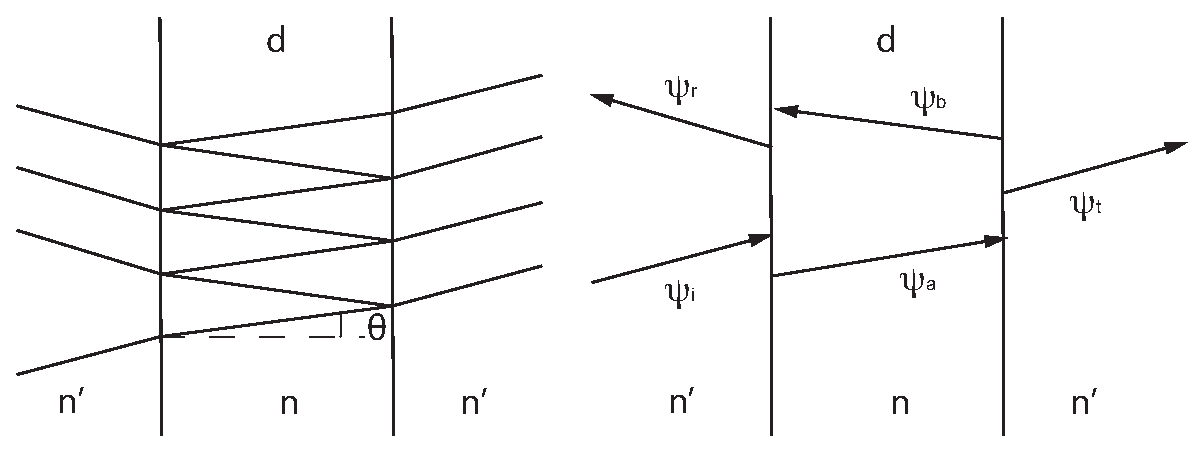
\psfig{file=fabry-perot-schematic.eps,width=0.95\textwidth}
  \caption{Schematic form of a Fabry-P\'erot interferometer. The light enters from the 
left and exits to the right (and left).}
  \label{fig:fabry-perot-schematic}
\end{figure}

A Fabry-P\'erot interferometry is based on trapping monochromatic light between two
highly reflecting surfaces. Let us consider the situation sketched in figure~\ref{fig:fabry-perot-schematic} where we have drawn two reflecting surfaces that are parallel and a distance $d$ apart. In between these plates there is a transparent medium with an index of refraction $n$, while outside the plates it is $n'$. Such a device is called an {\it etalon}. One example is a glass slab in air, another is a vacuum maintained between two glass mirrors. Suppose a plane wave with circular frequency $\omega$ is incident on one of the reflecting surfaces, where it is partially reflected and partially transmitted. The transmitted wave will propagate through to the second surface where it will be partially reflected and partially transmitted. The reflected portion will return to the first surface to be split, and so on. The resulting total fields in the slab
and beyond could be computed by summing the series of sequential reflections and transmission. Alternately one can proceed as below:

The series if summed will lead to five waves shown in the right panel of figure~\ref{fig:fabry-perot-schematic}: an incident wave ($\psi_i$), a reflected wave
($\psi_r$),  a transmitted wave ($\psi_t$), and two internal waves ($\psi_a,\psi_b$) 
with fields measured at the first surface. 

Introduce further reflection and transmission coefficients $r$ and $t$ for waves incident
on the slab from outside. Likewise, introduce $r'$ and $t'$ for waves incident on the slab
from inside. These coefficients are functions of the angles of incidence and the polarization. They can be computed using electromagnetic theory, but we need not do so here. 

\begin{figure}[h]
  \centering  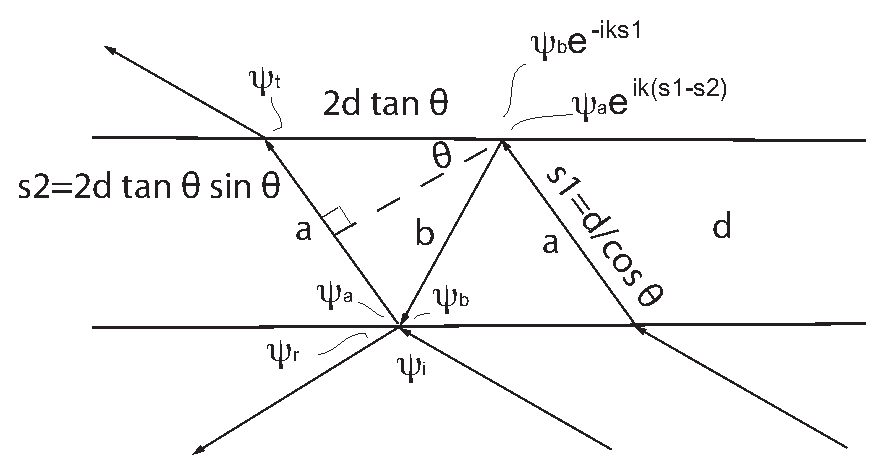
\psfig{file=fabry-phase-diff.eps,width=0.95\textwidth}
  \caption{Construction for calculating the phase differences across each slab for the
two internal waves in an etalon.}
  \label{fig:fabry-phase-diff}
\end{figure}

At the first surface we can write
\bea{eq:first-surface}
\psi_r&=&r\psi_i+t'\psi_b \nonumber \\
\psi_a&=&t\psi_i+r'\psi_b
\eea
\noindent
Geometry shows the the waves on the second surface are as in figure~\ref{fig:fabry-phase-diff}, and correspondingly the relationships between the ingoing and outgoing waves are 
\bea{eq:second-surface}
\psi_be^{-iks_1}&=&r'\psi_ae^{ik(s_1-s_2)} \nonumber \\
\psi_t&=&t'\psi_ae^{iks_1}
\eea
\noindent
where $k={n\omega/c}$ is the wave number in the slab and 
\[
s_1={d/\cos\theta},\qquad s_2=2d\tan\theta\sin\theta
\]
with $d$ the thickness of the slab and $\theta$ the angle that the wave fronts inside the
slab make to the slab's faces.

In solving for $\psi_t$ and $\psi_r$ as functions of $\psi_i$ we will need relations between the reflection and transmission coefficients. Consider the limit in which the
slab thickness $d\rightarrow 0$. In this limit $s_1=s_2=0$ and the slab must become
transparent so 
\[ \psi_r=0, \qquad \psi_t=\psi_i. \]
From the equations above we can then arrive at 
\be r'=-r, \qquad tt'-rr'=1. \label{eq:reciprocity-relations}\ee
Since there is no mechanism to produce a phase shift as the waves propagate across a 
perfectly sharp boundary, we can also expect that $r$, $r'$, $t$, and $t'$ are real. 

Returning to the case of $d\ne 0$, we find that by solving the equations~\ref{eq:first-surface} and \ref{eq:second-surface}, as well as the reciprocity relations~\ref{eq:reciprocity-relations} we can derive
\[ \psi_r={r(1-e^{i\phi})\over 1-r^2e^{i\phi}}\psi_i,\qquad
    \psi_t={(1-r^2)e^{i\phi}\over 1-r^2e^{i\phi}}\psi_i
\]
\noindent 
where
\[
\phi={2n\omega d\cos\theta/c}
\]

\begin{enumerate}
\setcounter{enumi}{\value{count}}
\item Derive the relations for $\psi_r$ and $\psi_t$ as functions of
  $r$, the incident field $\psi_i$ and the `angle' $\phi={2n\omega
    d\cos\theta/c}$. 
\setcounter{count}{\value{enumi}}
\end{enumerate}

\begin{figure}[h]
  \centering  \psfig{file=fabry-transmission.eps,width=0.95\textwidth}
  \caption{Transmission coefficient for an etalon as a function of the phase $\phi$ for 
reflectivities of $r=0.2$, $r=0.4$, and $r=0.9$.}
  \label{fig:fabry-transmission}
\end{figure}

It is very interesting to find the total reflection and transmission coefficients for the flux:
\bea{eq:reflection-transmission}
R&=&{\labs\psi_r\rabs^2\over\labs\psi_i\rabs^2}={2r^2(1-\cos\phi)\over 1-2r^2\cos\phi+r^4}\nonumber \\
T&=&{\labs\psi_t\rabs^2\over\labs\psi_i\rabs^2}={(1-r^2)^2\over 
 1-2r^2\cos\phi+r^4}
\eea
\noindent
From these expressions it is clear that
\[ R+T=1 \]
\noindent
which says that the energy flux reflected from the slab plus that transmitted is equal to that impinging on the slab. It is actually the reciprocity relations that have enforced this energy conservation.

Let us now introduce the finesse 
\[\cl{F}\equiv {\pi r/(1-r^2)}, \]
in terms of which
\[ T={1\over 1+({2\cl{F}/\pi})^2\sin^2{1\over 2}\phi} \]
\noindent
Suppose that the etalon is highly reflecting, so $r\simeq 1$. Then $\cl{F}$ is very large
and the transmissivity $T$ exhibits resonances. Unless $\sin{1\over 2}\phi$ is small, 
almost all the incident light is reflected by the etalon. The exception is when $\sin{1\over 2}\phi$ is small, then the total transmission can be large, even unity in the limit $\sin{1\over 2}\phi\rightarrow 0$. Notice that for large finesse, the half width of the resonance (the value of $\delta\phi\equiv\phi-\phi_{\rm resonance}$  where $T$ falls to $1/2$) is $\delta\phi_{1/2}={\pi/\cl{F}}$. The separation between the resonances, the
free spectral range, is $\delta\phi=\pi$, so the finesse is the ratio of the free spectral 
range to the resonance half width.

\begin{enumerate}
\setcounter{enumi}{\value{count}}
\item Compute the reflection $R$ and transmission $T$ {\bf flux}
  coefficients. 
\item Find the expression for the transmission coefficient in terms of
  the finesse. Using {\sc idl} plot $T$ as a function of $\phi$ with $r=0.2,0.4,0.9$.
\setcounter{count}{\value{enumi}}
\end{enumerate}

The etalon can be tuned to a particular frequency by varying either the slab width $d$ or the angle of incidence of the radiation (and thus $\theta$ inside the etalon). Either way very good chromatic resolving power can be achieved. One can say that waves with nearly the same frequencies are resolved by an etalon when the half power point of the transmission coefficient of one wave coincides with the half power point of the transmission coefficient of the other. {\it I.e.} using equation~\ref{eq:reflection-transmission} the phases for the two frequencies must differ by $d\phi\sim{2\pi/\cl{F}}$; and since $\phi={2n\omega d\cos\theta/c}$, the chromatic resolving power is 
\[
\cl{R}={\lambda\over\delta\lambda}={2\pi nd\over\lambda_{\rm vac}\delta\phi}
         ={2nd\cl{F}\over\lambda_{\rm vac}}
\]
\noindent
where $\lambda_{\rm vac}$ is the wavelength in vacuum --- {\it i.e.} outside the etalon. The finesse $\cl{F}$ can be regarded as a quality factor for the resonator. It is roughly the number of times a typical photon traverses the etalon before escaping. 
\end{document}